\documentclass{standalone}
\usepackage{tikz}
\usetikzlibrary{patterns, positioning}

\begin{document}
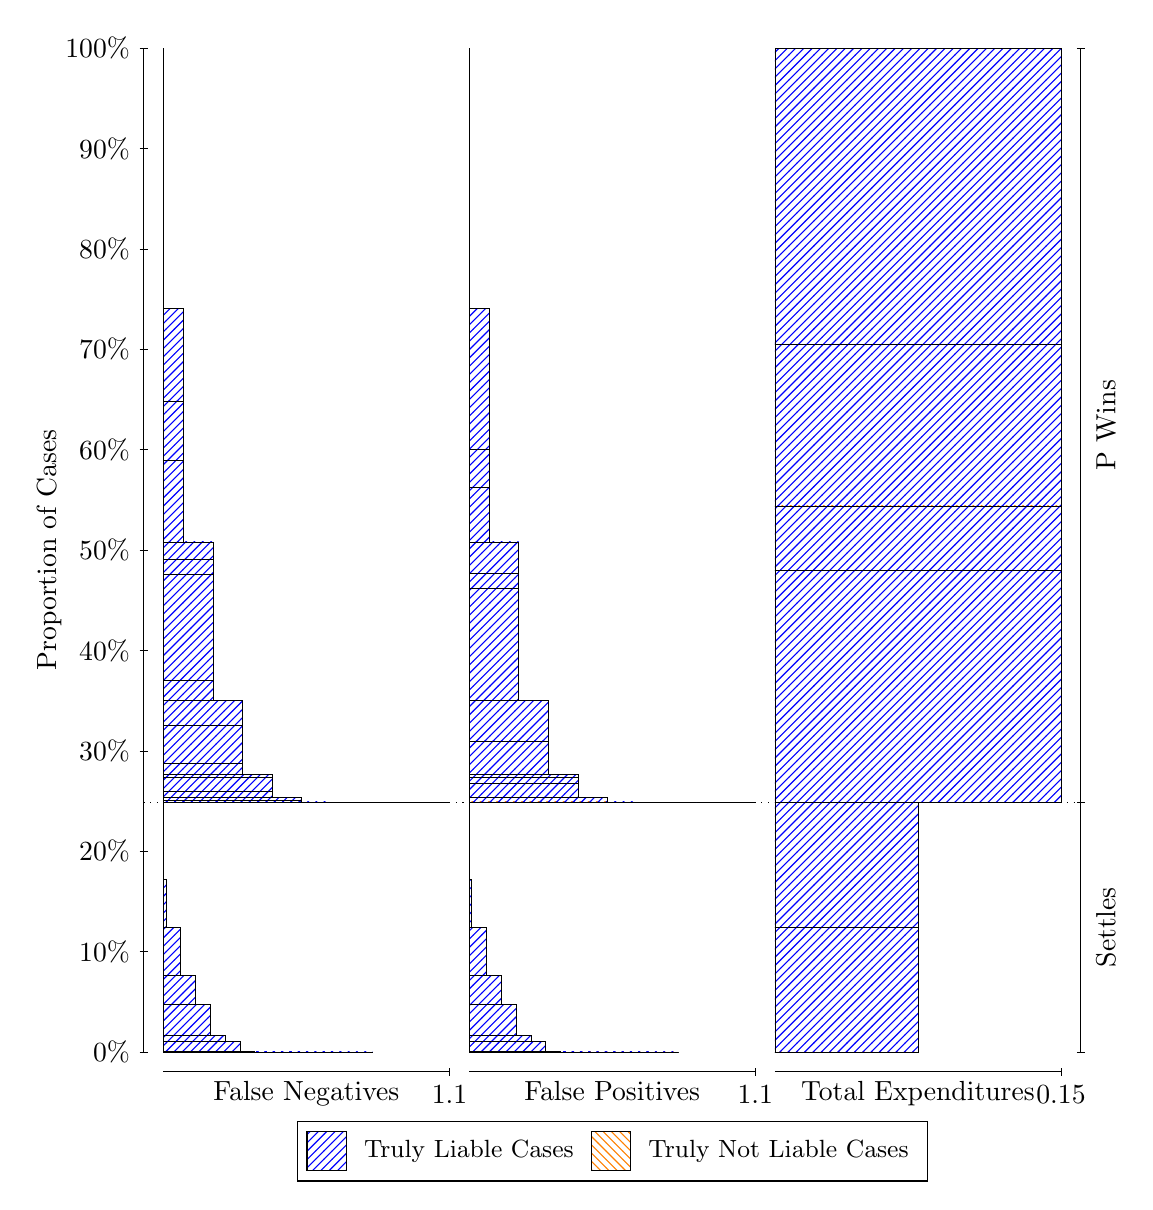
\begin{tikzpicture}
\draw[black, very thin] (1.5,1.75) -- (1.5,14.5);
\node[rotate=90, anchor=center] at (0.3, 8.125) {Proportion of Cases};
\draw[black, very thin] (1.45,1.75) -- (1.55,1.75);
\node[anchor=east] at (1.45, 1.75) {0\%};
\draw[black, very thin] (1.45,3.025) -- (1.55,3.025);
\node[anchor=east] at (1.45, 3.025) {10\%};
\draw[black, very thin] (1.45,4.3) -- (1.55,4.3);
\node[anchor=east] at (1.45, 4.3) {20\%};
\draw[black, very thin] (1.45,5.575) -- (1.55,5.575);
\node[anchor=east] at (1.45, 5.575) {30\%};
\draw[black, very thin] (1.45,6.85) -- (1.55,6.85);
\node[anchor=east] at (1.45, 6.85) {40\%};
\draw[black, very thin] (1.45,8.125) -- (1.55,8.125);
\node[anchor=east] at (1.45, 8.125) {50\%};
\draw[black, very thin] (1.45,9.4) -- (1.55,9.4);
\node[anchor=east] at (1.45, 9.4) {60\%};
\draw[black, very thin] (1.45,10.675) -- (1.55,10.675);
\node[anchor=east] at (1.45, 10.675) {70\%};
\draw[black, very thin] (1.45,11.95) -- (1.55,11.95);
\node[anchor=east] at (1.45, 11.95) {80\%};
\draw[black, very thin] (1.45,13.225) -- (1.55,13.225);
\node[anchor=east] at (1.45, 13.225) {90\%};
\draw[black, very thin] (1.45,14.5) -- (1.55,14.5);
\node[anchor=east] at (1.45, 14.5) {100\%};

\draw[black, very thin] (13.4,1.75) -- (13.4,14.5);
\draw[black, very thin] (13.35,1.75) -- (13.45,1.75);
\node[anchor=west] at (13.35, 1.75) {};
\draw[black, very thin] (13.35,4.9188) -- (13.45,4.9188);
\node[anchor=west] at (13.35, 4.9188) {};
\draw[black, very thin] (13.35,14.5) -- (13.45,14.5);
\node[anchor=west] at (13.35, 14.5) {};

\draw[black, very thin, pattern color=blue, pattern=north east lines] (1.75,1.75) rectangle (4.4116,1.75);
\draw[black, very thin, pattern color=blue, pattern=north east lines] (1.75,1.75) rectangle (4.0361,1.75);
\draw[black, very thin, pattern color=blue, pattern=north east lines] (1.75,1.75) rectangle (3.6606,1.75);
\draw[black, very thin, pattern color=blue, pattern=north east lines] (1.75,1.75) rectangle (3.5667,1.75);
\draw[black, very thin, pattern color=blue, pattern=north east lines] (1.75,1.75) rectangle (3.285,1.7502);
\draw[black, very thin, pattern color=blue, pattern=north east lines] (1.75,1.7502) rectangle (3.1911,1.7502);
\draw[black, very thin, pattern color=blue, pattern=north east lines] (1.75,1.7502) rectangle (2.9095,1.7576);
\draw[black, very thin, pattern color=blue, pattern=north east lines] (1.75,1.7576) rectangle (2.8156,1.7576);
\draw[black, very thin, pattern color=blue, pattern=north east lines] (1.75,1.7576) rectangle (2.7217,1.8797);
\draw[black, very thin, pattern color=blue, pattern=north east lines] (1.75,1.8797) rectangle (2.5339,1.9638);
\draw[black, very thin, pattern color=blue, pattern=north east lines] (1.75,1.9638) rectangle (2.4401,1.9639);
\draw[black, very thin, pattern color=blue, pattern=north east lines] (1.75,1.9639) rectangle (2.3462,2.3553);
\draw[black, very thin, pattern color=blue, pattern=north east lines] (1.75,2.3553) rectangle (2.1584,2.7222);
\draw[black, very thin, pattern color=blue, pattern=north east lines] (1.75,2.7222) rectangle (2.0645,2.7227);
\draw[black, very thin, pattern color=blue, pattern=north east lines] (1.75,2.7227) rectangle (1.9706,3.3344);
\draw[black, very thin, pattern color=blue, pattern=north east lines] (1.75,3.3344) rectangle (1.7829,3.9461);
\draw[black, very thin, pattern color=orange, pattern=north west lines] (1.75,3.9461) rectangle (1.75,3.9461);
\draw[black, very thin, pattern color=blue, pattern=north east lines] (1.75,3.9461) rectangle (1.75,4.9188);
\draw[black, very thin, pattern color=blue, pattern=north east lines] (1.75,4.9188) rectangle (5.3833,4.9188);
\draw[black, very thin, pattern color=blue, pattern=north east lines] (1.75,4.9188) rectangle (5.0078,4.9188);
\draw[black, very thin, pattern color=blue, pattern=north east lines] (1.75,4.9188) rectangle (5.0078,4.9188);
\draw[black, very thin, pattern color=blue, pattern=north east lines] (1.75,4.9188) rectangle (4.6323,4.9188);
\draw[black, very thin, pattern color=blue, pattern=north east lines] (1.75,4.9188) rectangle (4.6323,4.9188);
\draw[black, very thin, pattern color=blue, pattern=north east lines] (1.75,4.9188) rectangle (4.2567,4.9192);
\draw[black, very thin, pattern color=blue, pattern=north east lines] (1.75,4.9192) rectangle (4.2567,4.9193);
\draw[black, very thin, pattern color=blue, pattern=north east lines] (1.75,4.9193) rectangle (3.8812,4.9263);
\draw[black, very thin, pattern color=blue, pattern=north east lines] (1.75,4.9263) rectangle (3.5056,4.9422);
\draw[black, very thin, pattern color=blue, pattern=north east lines] (1.75,4.9422) rectangle (3.5056,4.9844);
\draw[black, very thin, pattern color=blue, pattern=north east lines] (1.75,4.9844) rectangle (3.1301,5.0558);
\draw[black, very thin, pattern color=blue, pattern=north east lines] (1.75,5.0558) rectangle (3.1301,5.2399);
\draw[black, very thin, pattern color=blue, pattern=north east lines] (1.75,5.2399) rectangle (3.1301,5.2798);
\draw[black, very thin, pattern color=blue, pattern=north east lines] (1.75,5.2798) rectangle (2.7546,5.4111);
\draw[black, very thin, pattern color=blue, pattern=north east lines] (1.75,5.4111) rectangle (2.7546,5.9002);
\draw[black, very thin, pattern color=blue, pattern=north east lines] (1.75,5.9002) rectangle (2.7546,6.2193);
\draw[black, very thin, pattern color=blue, pattern=north east lines] (1.75,6.2193) rectangle (2.379,6.4691);
\draw[black, very thin, pattern color=blue, pattern=north east lines] (1.75,6.4691) rectangle (2.379,7.8125);
\draw[black, very thin, pattern color=blue, pattern=north east lines] (1.75,7.8125) rectangle (2.379,8.0057);
\draw[black, very thin, pattern color=blue, pattern=north east lines] (1.75,8.0057) rectangle (2.379,8.2271);
\draw[black, very thin, pattern color=blue, pattern=north east lines] (1.75,8.2271) rectangle (2.0035,9.2671);
\draw[black, very thin, pattern color=blue, pattern=north east lines] (1.75,9.2671) rectangle (2.0035,10.019);
\draw[black, very thin, pattern color=blue, pattern=north east lines] (1.75,10.019) rectangle (2.0035,11.192);
\draw[black, very thin, pattern color=orange, pattern=north west lines] (1.75,11.192) rectangle (1.75,11.192);
\draw[black, very thin, pattern color=blue, pattern=north east lines] (1.75,11.192) rectangle (1.75,14.5);
\draw[black, very thin, pattern color=orange, pattern=north west lines] (5.6333,1.75) rectangle (8.295,1.75);
\draw[black, very thin, pattern color=blue, pattern=north east lines] (5.6333,1.75) rectangle (8.295,1.75);
\draw[black, very thin, pattern color=blue, pattern=north east lines] (5.6333,1.75) rectangle (7.9194,1.75);
\draw[black, very thin, pattern color=blue, pattern=north east lines] (5.6333,1.75) rectangle (7.5439,1.75);
\draw[black, very thin, pattern color=orange, pattern=north west lines] (5.6333,1.75) rectangle (7.45,1.75);
\draw[black, very thin, pattern color=blue, pattern=north east lines] (5.6333,1.75) rectangle (7.45,1.75);
\draw[black, very thin, pattern color=blue, pattern=north east lines] (5.6333,1.75) rectangle (7.1683,1.7502);
\draw[black, very thin, pattern color=blue, pattern=north east lines] (5.6333,1.7502) rectangle (7.0745,1.7502);
\draw[black, very thin, pattern color=blue, pattern=north east lines] (5.6333,1.7502) rectangle (6.7928,1.7576);
\draw[black, very thin, pattern color=blue, pattern=north east lines] (5.6333,1.7576) rectangle (6.6989,1.7576);
\draw[black, very thin, pattern color=orange, pattern=north west lines] (5.6333,1.7576) rectangle (6.605,1.7576);
\draw[black, very thin, pattern color=blue, pattern=north east lines] (5.6333,1.7576) rectangle (6.605,1.8797);
\draw[black, very thin, pattern color=blue, pattern=north east lines] (5.6333,1.8797) rectangle (6.4173,1.9638);
\draw[black, very thin, pattern color=blue, pattern=north east lines] (5.6333,1.9638) rectangle (6.3234,1.9639);
\draw[black, very thin, pattern color=blue, pattern=north east lines] (5.6333,1.9639) rectangle (6.2295,2.3552);
\draw[black, very thin, pattern color=blue, pattern=north east lines] (5.6333,2.3552) rectangle (6.0417,2.7221);
\draw[black, very thin, pattern color=blue, pattern=north east lines] (5.6333,2.7221) rectangle (5.9478,2.7227);
\draw[black, very thin, pattern color=blue, pattern=north east lines] (5.6333,2.7227) rectangle (5.854,3.3344);
\draw[black, very thin, pattern color=blue, pattern=north east lines] (5.6333,3.3344) rectangle (5.6662,3.9461);
\draw[black, very thin, pattern color=blue, pattern=north east lines] (5.6333,3.9461) rectangle (5.6333,4.9188);
\draw[black, very thin, pattern color=orange, pattern=north west lines] (5.6333,4.9188) rectangle (9.2667,4.9188);
\draw[black, very thin, pattern color=blue, pattern=north east lines] (5.6333,4.9188) rectangle (9.2667,4.9188);
\draw[black, very thin, pattern color=orange, pattern=north west lines] (5.6333,4.9188) rectangle (8.8911,4.9188);
\draw[black, very thin, pattern color=blue, pattern=north east lines] (5.6333,4.9188) rectangle (8.8911,4.9188);
\draw[black, very thin, pattern color=orange, pattern=north west lines] (5.6333,4.9188) rectangle (8.5156,4.9188);
\draw[black, very thin, pattern color=blue, pattern=north east lines] (5.6333,4.9188) rectangle (8.5156,4.9188);
\draw[black, very thin, pattern color=blue, pattern=north east lines] (5.6333,4.9188) rectangle (8.5156,4.9188);
\draw[black, very thin, pattern color=blue, pattern=north east lines] (5.6333,4.9188) rectangle (8.1401,4.9191);
\draw[black, very thin, pattern color=orange, pattern=north west lines] (5.6333,4.9191) rectangle (8.1401,4.9191);
\draw[black, very thin, pattern color=blue, pattern=north east lines] (5.6333,4.9191) rectangle (8.1401,4.9193);
\draw[black, very thin, pattern color=orange, pattern=north west lines] (5.6333,4.9193) rectangle (7.7645,4.9193);
\draw[black, very thin, pattern color=blue, pattern=north east lines] (5.6333,4.9193) rectangle (7.7645,4.9263);
\draw[black, very thin, pattern color=orange, pattern=north west lines] (5.6333,4.9263) rectangle (7.389,4.9263);
\draw[black, very thin, pattern color=blue, pattern=north east lines] (5.6333,4.9263) rectangle (7.389,4.9844);
\draw[black, very thin, pattern color=orange, pattern=north west lines] (5.6333,4.9844) rectangle (7.0134,4.9844);
\draw[black, very thin, pattern color=blue, pattern=north east lines] (5.6333,4.9844) rectangle (7.0134,5.1601);
\draw[black, very thin, pattern color=blue, pattern=north east lines] (5.6333,5.1601) rectangle (7.0134,5.2348);
\draw[black, very thin, pattern color=blue, pattern=north east lines] (5.6333,5.2348) rectangle (7.0134,5.2798);
\draw[black, very thin, pattern color=orange, pattern=north west lines] (5.6333,5.2798) rectangle (6.6379,5.2798);
\draw[black, very thin, pattern color=blue, pattern=north east lines] (5.6333,5.2798) rectangle (6.6379,5.7006);
\draw[black, very thin, pattern color=blue, pattern=north east lines] (5.6333,5.7006) rectangle (6.6379,6.2193);
\draw[black, very thin, pattern color=orange, pattern=north west lines] (5.6333,6.2193) rectangle (6.2624,6.2193);
\draw[black, very thin, pattern color=blue, pattern=north east lines] (5.6333,6.2193) rectangle (6.2624,7.6373);
\draw[black, very thin, pattern color=blue, pattern=north east lines] (5.6333,7.6373) rectangle (6.2624,7.8305);
\draw[black, very thin, pattern color=blue, pattern=north east lines] (5.6333,7.8305) rectangle (6.2624,8.2271);
\draw[black, very thin, pattern color=blue, pattern=north east lines] (5.6333,8.2271) rectangle (5.8868,8.9226);
\draw[black, very thin, pattern color=orange, pattern=north west lines] (5.6333,8.9226) rectangle (5.8868,8.9226);
\draw[black, very thin, pattern color=blue, pattern=north east lines] (5.6333,8.9226) rectangle (5.8868,9.4);
\draw[black, very thin, pattern color=blue, pattern=north east lines] (5.6333,9.4) rectangle (5.8868,11.192);
\draw[black, very thin, pattern color=blue, pattern=north east lines] (5.6333,11.192) rectangle (5.6333,14.5);
\draw[black, very thin, pattern color=orange, pattern=north west lines] (9.5167,1.75) rectangle (11.333,1.75);
\draw[black, very thin, pattern color=blue, pattern=north east lines] (9.5167,1.75) rectangle (11.333,3.3338);
\draw[black, very thin, pattern color=orange, pattern=north west lines] (9.5167,3.3338) rectangle (11.333,3.3338);
\draw[black, very thin, pattern color=blue, pattern=north east lines] (9.5167,3.3338) rectangle (11.333,4.9188);
\draw[black, very thin, pattern color=orange, pattern=north west lines] (9.5167,4.9188) rectangle (13.15,4.9188);
\draw[black, very thin, pattern color=blue, pattern=north east lines] (9.5167,4.9188) rectangle (13.15,7.8628);
\draw[black, very thin, pattern color=orange, pattern=north west lines] (9.5167,7.8628) rectangle (13.15,7.8628);
\draw[black, very thin, pattern color=blue, pattern=north east lines] (9.5167,7.8628) rectangle (13.15,8.6853);
\draw[black, very thin, pattern color=orange, pattern=north west lines] (9.5167,8.6853) rectangle (13.15,8.6853);
\draw[black, very thin, pattern color=blue, pattern=north east lines] (9.5167,8.6853) rectangle (13.15,10.734);
\draw[black, very thin, pattern color=orange, pattern=north west lines] (9.5167,10.734) rectangle (13.15,10.734);
\draw[black, very thin, pattern color=blue, pattern=north east lines] (9.5167,10.734) rectangle (13.15,14.5);
\draw[black, dotted] (1.5,4.9188) -- (13.4,4.9188);
\draw[black, very thin] (1.75,1.5) -- (5.3833,1.5);
\node[anchor=north] at (3.5667, 1.5) {False Negatives};
\draw[black, very thin] (5.3833,1.45) -- (5.3833,1.55);
\node[anchor=north] at (5.3833, 1.45) {1.1};

\draw[black, very thin] (5.6333,1.5) -- (9.2667,1.5);
\node[anchor=north] at (7.45, 1.5) {False Positives};
\draw[black, very thin] (9.2667,1.45) -- (9.2667,1.55);
\node[anchor=north] at (9.2667, 1.45) {1.1};

\draw[black, very thin] (9.5167,1.5) -- (13.15,1.5);
\node[anchor=north] at (11.333, 1.5) {Total Expenditures};
\draw[black, very thin] (13.15,1.45) -- (13.15,1.55);
\node[anchor=north] at (13.15, 1.45) {0.15};

\node[black, centered, rotate=90] at (13.72, 3.3344) {Settles};
\node[black, centered, rotate=90] at (13.72, 9.7094) {P Wins};

\draw (7.449999999999999,1.5) node[draw=none] (baseCoordinate) {};
\begin{scope}[align=center]
        \matrix[scale=0.5, draw=black, below=0.5cm of baseCoordinate, nodes={draw}, column sep=0.1cm]{
            \node[rectangle, draw, minimum width=0.5cm, minimum height=0.5cm, pattern=north east lines, pattern color=blue] {}; &
            \node[draw=none, font=\small] (B) {Truly Liable Cases}; &
            \node[rectangle, draw, minimum width=0.5cm, minimum height=0.5cm, pattern=north west lines, pattern color=orange] {}; &
            \node[draw=none, font=\small] (B) {Truly Not Liable Cases}; \\
            };
\end{scope}

\end{tikzpicture}
\end{document}